
\newpage
\section{Divisor Theory}
\label{sec:ch1.divisiors}

% Rational functions
Before we dive into the topic om divisors more detail, we first recall how quotients of polynomials behaves when two variables are represents points on an elliptic curve based on \cite{lynn2007implementation}.  Let $\mathbb{F}_{q^k}[X, Y]$ denote the ring of polynomials in variables $X, Y$ with  with coefficients in $\FF_{q^k}$. Furthermore assume we will define $E$ elliptic curve with  $Y^2 = X^3 + aX + b$ over $\mathbb{F}_{q^k}$. Then $E(X, Y)$ can be written as the polynomial $Y^2 - X^3 - aX - b$. 

In accordance with \cite{lynn2007implementation}  one can show that a polynomial $f$ satisfies $f(X, Y) = 0$ $E(X, Y) = 0$ if and only if $f(X, Y)$ is a multiple of $E(X, Y)$. This means that from all the possible polynomials we consider exactly only two of them to be equivalent if they take the same values on all points of $E$, denoted as $\mathbb{F}_{q^k}[E] = \mathbb{F}_{q^k}[X, Y]_{E(X,Y)}$. 

This observation provides us with the idea that every element $f(X, Y)$ in $\mathbb{F}_{q^k}[E]$ can be written in the form $f_x(X)+Yf_y(X)$ for polynomials
$f_x, f_y \in \mathbb{F}_{q^k}[X]$ because we may replace $Y^2$ by $X^3 + aX + b$. Precisely, if we define $\mathbb{F}_{q^k}(E)$ to be the field of fractions of $\mathbb{F}_{q^k}[E]$, then the elements of $\mathbb{F}_{q^k}(E)$ can be written in the form $f(X, Y)/g(X, Y)$ where $f, g$ are polynomials in two variables $X, Y$ and $g$ is not a multiple of $E$.

Recall the naming conventions from \cite{Menezes1993},  we say that a rational function $f \in K(E)$ on an elliptic curve $E$ have a \textit{zero} at a point $P \in E$ if $f(P) = 0$ and a \textit{pole} at $P$ if $f(P) = \infty$. 
% Zeroes and Poles
Following the previously outlined idea, it can be noted that the \textit{zeroes} are the roots of $f$ and the poles are the roots of $g$, therefore $f/g$ is  determined up to a constant by its zeroes and poles and their multiplicities. Suppose the zeroes and poles are denoted with $\alpha_1, \ldots, \alpha_n$. Let $a_1, \ldots, a_n$ denote the multiplicites  where $\alpha_i$ is a zero of multiplcity $a_i$. We also consider a zero of negative multiplicity $a_i$ to be a pole of multiplicity as $-a_i$. 

Then we write $f(X)/g(X)$ by multiplying equations of appropriate vertical lines:
\insertEquationEnvironmentWithLabel{
f(X)/g(X) = (X - \alpha_i)^{a_i}}{eq:rationalverticallines}

The main advantage of the generalization shown in \refEquation{eq:rationalverticallines} is that
one can view roots of a polynomial $f$ as places where the curve $Y = f(X)$ intersects
with the curve $Y = 0$. Consequently, we can further generalize by replacing $Y = 0$ with an elliptic curve. Thus we can call the points of intersection between $f(X, Y)$ and $E$ zeroes of $f$, where $f(X, Y) \in \mathbb{F}_{q^k}[E]$.  

However, similarly as before, complications will occur due to the point at infinity. We already presented \refSection{ssec:ch01.PointAtInfinityInProjectiveSpace} how one may use projective coordinates to handle the point at infinity. Now, building upon the technique presented before and in conjunction with the idea generalized in \refEquation{eq:rationalverticallines} it turns out that every line $\alpha X + \beta Y + \gamma$ that intersects a given elliptic curve $E$ has a pole at $\mathFormulaEllipticCurvePointAtInfinity$ of some multiplicity. 

To describe the multiplicities at zeroes and poles one can take advantage by introducing the uniformizing parameter $d$ for $P$, based on \cite{menezes2004ECC}.  Given all $P \in E$ there exists a rational function $u \in \overline{K}(E)$, $u(P) = 0$, such that if $f \in \overline{K}(E)^{*}$, then
\insertEquationEnvironmentWithLabel{f = u^{d}s}{eq:uniformizingparameter}
 
, where $s \in \overline{K}(E)$, $s(P) \neq 0, \infty$.  
The function $u$  in \refEquation{eq:uniformizingparameter} called a \textit{uniformizing parameter} for $P$, where the integer $d$ does not depend on the choice of $u$.  However, one question arises regarding how to choose the uniformizing parameter. To answer the question, we can distinguish between three different cases using \refEquation{eq:uniformizingparameter} and \textit{Theorem 2.22} from \cite{Menezes1993} as follows in \textit{Example \ref{example:uniformizingparameter}}. 


\begin{example}[Distinct cases for the uniformizing parameter.]
	\label{example:costofuniformizingparam}
	Given $E: y^2 = x^3 + ax +b$ over finite field $K = \mathbb{F}_q$, with $\operatorname{char}(K) \neq 2,3$. Refer to \refCodeSnippet{code:example.uniformizingparameter} in \refApxCode{apx_implementation:ch1.divisiors}
	
	\insertListEnvironment{
		\addListItem{Let $P = (c, d) \notin E[2]$. Then tangent line to  $E$ evaluated at $P$ is as follows:
			\[(-3c^{2} - a)(x - c) + 2d(y - d) = 0\],
			Since $d \neq 0$, a uniformizing parameter for $P$ is $u = x - c$.
			}
	
		\addListItem{Let $P = (c, 0) \in E$ be a point of order $2$. The tangent line to $E$ evaluated at $P$ is as follows:
		\[(-3c^{2} - a)(x - c) = 0.\]
		}
		\addListItem{To find a suitable uniformizing parameter for \mathFormulaEllipticCurvePointAtInfinity, we recall the coordinate substitution technique presented in \refSubsection{ssec:ch01.PointAtInfinityInProjectiveSpace}. First, 
		we choose the affine coordinates as $v = X/Y;~ w =Z/Y$, therefore the $E$ equation is transformed to $f(v,w)=v^3 + avw^2 + bw^3 -w = 0$. We note, that $\BigO = (0,0)$ using $(v,w)$-coordinate representation, thus:
			\insertListEnvironment{
			\item First, $\partials{f}{v}(\BigO)=0$ and $\partials{f}{w}(\BigO)=-1$, thus the equation 			of the tangent line to $E$ evaluated at $\BigO$ is $w=0$, 
			\item Secondly, the line $v = 0$ passes through $\BigO$ and is not the tangent line at $\BigO$, 
			\item Lastly, reverting back to the original $(x, y)$ coordinates we found that $u = x/y$  is a uniformizing parameter for $\BigO$.
			}
		}
	}
	\label{example:uniformizingparameter}
\end{example}

For instance, if a vertical line (represented as $X - \alpha$) intersects the $E$ elliptic curve  then it has a pole at $\mathFormulaEllipticCurvePointAtInfinity$ of multiplicity $2$. Secondly, if a non-vertical line (represented as $\alpha X + \beta Y + \gamma$) intersects $E$ then it has a pole of multiplicity $3$ at $\mathFormulaEllipticCurvePointAtInfinity$.  Using the just introduced notation in \refEquation{eq:uniformizingparameter}, we can formulate the order of $f$ at $P$  as $\operatorname{ord}_{P}(f) = d$. Therefore the point $P$ is a \textit{zero} of $f$ if and only if $\operatorname{ord}_{P}(f) > 0$, in case its multiplicity is defined to be
$\operatorname{ord}_{P}(f)$. On the other hand,  the point $P$ is a\textit{ pole} of $f$ if and only if $\operatorname{ord}_{P}(f) < 0$, then its multiplicity is defined to be $-\operatorname{ord}_{P}(f)$.
% Divisors from Costello

To make our case easier, we will introduce the concept of divisors, which is standard way to notate zeroes, poles and their multiplicities, or orders referring to \cite{lynn2007implementation}.  Given the scenario where we wish to record zeroes and poles $P_1, \ldots, P_n$ of orders $a_1, \ldots, a_n$ (where $P_i$ is a zero of
order $a_i$ if $a_i > 0$ and is a pole of order $-a_i$ otherwise, with generalization of $ord_P$ notation), then we represent the divisor as follows in \refEquation{eq:divisorwithpolesandzeroes}: 

\insertEquationEnvironmentWithLabel{D = a_1\langle P_1\rangle + \cdots + a_n\langle P_n\rangle}{eq:divisorwithpolesandzeroes}


With the notation introduced in \ref{eq:divisorwithpolesandzeroes},  if we add the divisors of two functions together, then the resulting divisor reflects the zeroes and poles of the product of the two functions.  Similarly, given the scenario where $D$ given the divisor with zeros and poles $P_1, \ldots, P_n$ of multiplicities $a_1, \ldots, a_n$. Then we can construct $D$ as follows in \ref{eq:divisorsasmultiplicities}:

\insertEquationEnvironmentWithLabel{
D = (P_1)^{a_1} \cdots (P_n)^{a_n}}{eq:divisorsasmultiplicities}


%For the rest of this section we examine the divisors in more detail based on \cite{theory.pairings.for.beginners}. But first, we relax our notation as follows: for the elliptic curve group law from now $+$ will be used instead of $\oplus$, while for inverse of the point $-$ will be used instead of $\ominus$. e.g: $-P$ instead of $\ominus \ P$

We note, that the following statements apply to all curves \mathFormulaObject{C} over any perfect field \mathFormulaFieldArbitrary and it's closure \mathFormulaFieldArbitraryClosure, however,
for now we place the discussion in our context and specialise to the case where \mathFormulaObject{C} is an elliptic curve \mathFormulaEllipticCurve{E} defined over a finite field as formulated by \mathFormulaTwoSidesEqual{\mathFormulaFieldArbitrary}{\FieldFq} as before. 

%\todo{cite Gal05}
%We will essentially just be expanding on the more concise section found in Galbraith's chapter \cite{} however, we only focus on what we need to describe elliptic curve pairings.

%The important concept of divisors on curves will be introduced in  \refSection{ssec:ch1.divisiors.classgroupandriemanroch}, their particular usefulness when used to describe functions on curves, since such a function is well defined (up to constant) by its points of intersection with a curve, and these are precisely what the divisor of the function encapsulates. After we defined the divisor class group of a (hyperelliptic) curve and discussed that for the case of elliptic curves, there is a bijection between this group and the set of points on the curve, so that we can simply talk about group elements as points
%on. Lastly we further illustrated several useful properties and
%theorems that play a big role in the realm of algebraic geometry, most notably
%the Riemann-Roch theorem and Weil reciprocity.

% --------------------------------------------



Using the definition of divisor (denoted by \mathFormulaDivisor ) on \mathFormulaEllipticCurve{E} is also a convenient way to denote the formal sum of multi-set of points on \mathFormulaEllipticCurve{E} with finitely many zeroes (\mathFormulaIsInSet{n_P}{\ZZ} ) as written in \refEquation{eq:ch1.divisorformalsum}: 

\insertEquationEnvironmentAlignedWithLabel{
	\mathFormulaTwoSidesEqual{\mathFormulaDivisor}{
		\mathFormulaSumFromTo{n_{\mathFormulaEllipticCurvePoint{P}}(\mathFormulaEllipticCurvePoint{P})}{\mathFormulaIsInSet{\mathFormulaEllipticCurvePoint{P}}{\mathFormulaEllipticCurvePar{E}{\mathFormulaAlgebraicClosureOf{\FieldF}}_q}}{}
	}
}{eq:ch1.divisorformalsum}	

We call the summarization in \refEquation{eq:ch1.divisorformalsum} formal because the parentheses  around \mathFormulaEllipticCurvePoint{P} and the absence of square parentheses around the  \mathFormulaObject{n_{\mathFormulaEllipticCurvePoint{P}}} is differentiates from the notation of the actual sum of points on \mathFormulaEllipticCurve{E} (see  \refSection{ssec:ch1.EllipticCurveGroupLaw}), where the square brackets denoted the sum of points using the group law.  The set of all divisors on \mathFormulaEllipticCurve{E} is thereby denoted by \mathFormulaDivisorOfPar{E}{\mathFormulaAlgebraicClosureOf{\FieldF}}. Also, the set of all divisors forms a group, where addition of divisors is natural, and the identity is the
divisor with all  \mathFormulaTwoSidesEqual{n_\mathFormulaEllipticCurvePoint{P}}{0}, where the zero divisor  \mathFormulaIsInSet{0}{\mathFormulaDivisorOfPar{E}{\mathFormulaAlgebraicClosureOf{\FieldF}}}
.    In addition, we interpret the degree of a divisor  denoted by \EquationDegreeOfDivisor, and the 
%the support of \mathFormulaDivisor (denoted by \mathFormulaSupportOf{\mathFormulaDivisor}).
the set of support can be understood as \mathFormulaTwoSidesEqual{\mathFormulaSupportOf{\mathFormulaDivisor}}{\{ \mathFormulaTwoSidesNotEqual{ P \in E( \mathFormulaAlgebraicClosureOf{\FieldF}_q) :n_P}{0}\}}.

\begin{example}[Properties of divisors.]
	% Costello book 3.0.1 script
	Consider $P,Q,R,S \in E(\overline{\FieldF}_q)$. Let $D_1 = 2(P) - 3(Q)$ and $D_2 = 3(Q) + (R) - (S)$, thus the degree of divisors: $Deg(D_1) = 2-3=-1$, and $Deg(D_2) = 3+1 -1 = 3$ respectively. The sum of divisors equals to $D_1 + D_2 = 2(P) + (R) - (S)$, furthermore $Deg(D_1 + D_2) = Deg(D_1) + Deg(D_2) = 2$. The supports are $\mathFormulaSupportOf{D_1} = \{P,Q\}$, $\mathFormulaSupportOf{D_2} = \{Q,R,S\}$. The sum of the support  then equals to $\mathFormulaSupportOf{D_1 + D_2} = \{P,R,S\}$.
\label{example:divisorsupportsum}	
\end{example}


Let $f$ denotes the the function associating divisors on \mathFormulaEllipticCurve{E} convenient way to write down the intersection points (and their multiplicities) of $f$ and \mathFormulaEllipticCurve{E}. \mathFormulaOrderOfWithIndex{f}{P} count
the multiplicity of $f$ at \mathFormulaEllipticCurvePoint{P} which is positive if $f$ has  zero at \mathFormulaEllipticCurvePoint{P} and negative if $f$ has a pole at \mathFormulaEllipticCurvePoint{P}. Using the just introduced notation the divisor of a function $f$ as $(f)$ and it is defined as the divisor as can be followed in \refEquation{eq:ch1.divisoroffunctionf}

\insertEquationEnvironmentWithLabel{
	(f) = \sum_{P \in E(\mathFormulaAlgebraicClosureOf{\FieldF}_q)}^{} \mathFormulaOrderOfWithIndex{f}{P}(P)
}{eq:ch1.divisoroffunctionf}

In \refSection{ssec:ch1.explicitformulaforgrouplaw} we've already seen examples of functions on \mathFormulaEllipticCurve{E} used in the chord-and-tangent rule, and it is natural that we are really only interested in the points of intersection of \mathFormulaObject{\ell} and \mathFormulaEllipticCurve{E}, which is exactly what the divisor (\mathFormulaObject{\ell}) tells us.

\begin{example}[Illustrative example based on \refFigure{fig:divisorlintersects}.]
%% example 3.0.2  + code ide

As an illustrative example we use \refFigure{fig:divisorlintersects}, where the chord \mathFormulaObject{\ell} intersects  \mathFormulaEllipticCurve{E} in \mathFormulaEllipticCurvePoint{P}, \mathFormulaEllipticCurvePoint{Q} and \mathFormulaEllipticCurvePoint{-(P+Q)}, all with multiplicity $1$.  We can also observe that  \mathFormulaObject{\ell} intersects \mathFormulaEllipticCurve{E} with multiplicity $-3$ at \mathFormulaEllipticCurvePointAtInfinity, since \mathFormulaObject{\ell} has a pole of order $3$ at \mathFormulaEllipticCurvePointAtInfinity. Thus, \mathFormulaObject{\ell} has divisor  $(l)=(P)+(Q) + (-(P+Q))-3(\BigO)$. Refer to \refCodeSnippet{code:divisorbasedondrawing} in \refApxCode{apx_implementation:ch1.divisiors}.
\label{example:divisorbasedondrawing}	
\end{example}




\begin{figure}[!htb]
	\centering
	\begin{minipage}{.5\textwidth}
		\centering
		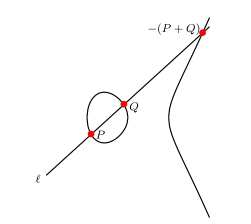
\includegraphics[width=0.8\linewidth]{98_Pictures/Chapter_01/divisorlintersects}
		\caption{The divisor $(l)$ intersects  $E$. $(l)=(P)+(Q) + (-(P+Q))-3(\BigO)$}
		\label{fig:divisorlintersects}
 \end{minipage}%
	\begin{minipage}{0.5\textwidth}
		\centering
		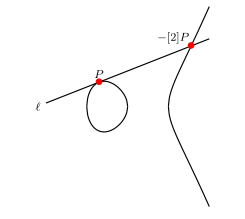
\includegraphics[width=0.8\linewidth]{98_Pictures/Chapter_01/divisorlintersectsppointdoubling}
		\caption{Line $\ell$ intersection with $P$ point-doubling. $(\ell)= 2 (P) + (-[2]P) - 3 (\BigO)$}
		\label{fig:divisorlintersectsppointdoubling}
	\end{minipage}%
\end{figure}




\begin{example}[Illustrative example based on \refFigure{fig:divisorlintersectsppointdoubling}.]
Another case is, where the tangent \mathFormulaObject{\ell} intersects \mathFormulaEllipticCurve{E} with multiplicity $2$ at \mathFormulaEllipticCurvePoint{P}, with multiplicity $1$ at $-[2] \mathFormulaEllipticCurvePoint{P}$, and with multiplicity $-3$ at \mathFormulaEllipticCurvePointAtInfinity~ as can be seen \refFigure{fig:divisorlintersectsppointdoubling}, as in this case $(l)=2(P) + (-[2]P) - 3(\BigO)$.
Refer to \refCodeSnippet{code:divisorlintersectsppointdoubling} in \refApxCode{apx_implementation:ch1.divisiors}.
\label{example:divisorlintersectsppointdoubling}
\end{example}





%\todo{Example 3.0.2 pseudo kod a pelda alapjan + kod reszlet az appendix-be}
In both cases, as depicted on \textit{\ref{fig:divisorlintersects}} and \refFigure{fig:divisorlintersectsppointdoubling} we have \mathFormulaTwoSidesEqual{\mathFormulaDegreeOfPar{\ell}}{0}. 
As illustrated, for any function $f$ on \mathFormulaEllipticCurve{E} we will always have \mathFormulaTwoSidesEqual{\mathFormulaDegreeOfPar{\ell}}{0} as stated in \textit{Theorem 7.7.1} \cite{Gal12}. This property follows from observing that the degree of the affine equation that solves for the zeros of $f$ on \mathFormulaEllipticCurve{E}  matches the degree of the projective equation that determines the multiplicity of the pole of $f$ at \mathFormulaEllipticCurvePointAtInfinity. This corresponds to the projective version of $f=g/h$) where $g$ and $h$ both have the same degree as $f$.

The algebra between functions naturally translates across to the algebra between their divisors, meaning, that \mathFormulaTwoSidesEqual{(fg)}{(f) + (g)} and \mathFormulaTwoSidesEqual{(f/g)}{(f)-(g)} therefore \mathFormulaTwoSidesEqual{(f)-(g)}{0} 
if and only if $f$ is constant.  For instance, given \mathFormulaTwoSidesEqual{(f)}{(g)} then \mathFormulaTwoSidesEqual{(f/g)}{0}, thus if $f$ is a constant multiple of $g$, it  means consequently that the divisor $(f)$ determines $f$ up to non-zero scalar multiples.

\begin{example}
From \textit{Example \ref{example:divisorbasedondrawing}} we know that three zeros (counting multiplicities) will always arise from substituting
$\ell : y = \lambda x + \nu$ into $E/\mathbb{F}_q : y^{2} = x^{3} + ax + b$. However, during the example we only considered $\ell$ on the affine curve $E \cap \mathbb{A}^{2}$, where $\ell$ has no poles.   To consider the case $\ell$ on $E$ at $O = (0 : 1 : 0)$ (in $\mathbb{P}^{2}(\mathbb{F}_q)$), we need to apply $x = X/Z$ and $y = Y/Z$ substitutions which gives $\left(\dfrac{\lambda X + \nu Z}{Z}\right)^2 = \left( \dfrac{X}{Z} \right)^3 + a \left( \dfrac{X}{Z}  \right) + b $, therefore we have a pole of order $3$ when $Z = 0$. 
\label{example:polecountinginprojectivespace}
\end{example}

In the following  \refSubsection{ssec:ch1.divisiors.classgroupandriemanroch} we will now focus on divisor class groups, subgroups of divisors, as well the implications arising from their group structures.

\newpage

\subsection{The divisor class group and consequence of the Riemann-Roch Theorem}
\label{ssec:ch1.divisiors.classgroupandriemanroch}
%The subgroups of divisors will be denoted as \EquationDivisorOnEOverFieldFq.  
The set of degree zero divisors forms a proper subgroup, which we write as \mathFormulaDivisorProperSubgroupOf{0}{E}, constructed as   \mathFormulaSetOfDivisors{D}{0}.  We will call \mathFormulaDivisor~ \textit{principal} divisor, if a divisor \mathFormulaDivisor~ on \mathFormulaEllipticCurve{E} and the set of principal divisors naturally form a group, written as \mathFormulaPrincipalDivisor{E}. Principal divisors furthermore have degree zero, but there are also degree zero divisors that are not the divisors of a function, so the degree zero subgroup is strictly larger than the principal divisors i.e \mathFormulaIsSubsetOf{\mathFormulaPrincipalDivisor{E}}{\mathFormulaDivisorWithDegreeOf{E}{0}}





There is, however, an extra condition on elements of \mathFormulaDivisorWithDegreeOf{E}{0}. Namely, \mathFormulaTwoSidesEqual{\mathFormulaDivisor}{\sum_{P}^{} n_P(P) \in \mathFormulaDivisorWithDegreeOf{E}{0}} is principal if and only if \mathFormulaTwoSidesEqual{\sum_{P}^{} [n_P] P }{\mathFormulaEllipticCurvePointAtInfinity} on \mathFormulaEllipticCurve{E} in accordance with \textit{Theorem IX 2.} from \cite{Gal05}. Before we define the divisor class group of E, we look at the important notion
of divisor equivalence in \mathFormulaDivisorOfPar{E}{}. We call the divisors \mathFormulaDivisorWithIndex{1} and \mathFormulaDivisorWithIndex{2} equivalent (denoted as \mathFormulaTwoSidesSimilar{\mathFormulaDivisorWithIndex{1}}{\mathFormulaDivisorWithIndex{2}})
, if \mathFormulaTwoSidesEqual{\mathFormulaDivisorWithIndex{1}}{\mathFormulaDivisorWithIndex{2} + (f)} for some function $f$. 

The \textit{divisor class group} (or  \textit{Picard group} ) of $E$ is defined as the quotient group  as can be followed \refEquation{eq:ch1.picardgroupdefinition}.

\insertEquationEnvironmentWithLabel{
	\mathFormulaTwoSidesEqual{\mathFormulaPicardGroupWithIndexPar{E}{0}}{\mathFormulaDivisorGroupWithIndexPar{E}{0}/
		\mathFormulaPrincipalDivisor{E}}
}{eq:ch1.picardgroupdefinition}

\refEquation{eq:ch1.picardgroupdefinition} means that  the divisor class group is the group of all degree zero divisors modulo the principal divisors on \mathFormulaEllipticCurve{E}. Let us consider \refExample{example:grouplawwithdivisors} with the just introduced notion to describe the elliptic curve group law in terms of divisors, following from \textit{Chapter IX.2} \cite{Gal05}.

\begin{example}[Describe the elliptic curve group law in terms of divisors.]
	% Example 3.1.2 <- Costello
	Referring back go \textit{Figure} or 2.6 in the case that $Q=P$ the line \mathFormulaObject{\ell} joining \mathFormulaEllipticCurvePoint{P},\mathFormulaEllipticCurvePoint{Q} has divisor:
	\mathFormulaTwoSidesEqual{(\ell)}{(\mathFormulaEllipticCurvePoint{P}) + (\mathFormulaEllipticCurvePoint{Q})+ (-\mathFormulaEllipticCurvePoint{R}) - 3 (\mathFormulaEllipticCurvePointAtInfinity)}, whilst the vertical line $v=x-x_R$ has divisor \mathFormulaTwoSidesEqual{(v)}{(-R) + (R) - 2(\mathFormulaEllipticCurvePointAtInfinity)}. The quotient $\dfrac{\ell}{v}$ has divisor \mathFormulaTwoSidesEqual{(\dfrac{\ell}{v})}{(P) + (Q) - (R) - (\mathFormulaEllipticCurvePointAtInfinity) }. Thus the equation $R = P + Q$ on $E$ is the same as the divisor equality $(R) - (\mathFormulaEllipticCurvePointAtInfinity) = (P) - (\mathFormulaEllipticCurvePointAtInfinity) + (Q) - (\mathFormulaEllipticCurvePointAtInfinity) - \left(\dfrac{\ell}{v}\right)$.
	
	Now, to concretely connect this back to \refEquation{eq:ch1.picardgroupdefinition} both $(R) - (\mathFormulaEllipticCurvePointAtInfinity)$ and $(P) + (Q) - 2 (\mathFormulaEllipticCurvePointAtInfinity)$ are in \mathFormulaDivisorGroupWithIndexPar{E}{0}, thus they represent the same class in \mathFormulaPicardGroupWithIndexPar{E}{0} because the divisor is principal, and therefore zero in \mathFormulaPicardGroupWithIndexPar{E}{0}.
	
	\label{example:grouplawwithdivisors}
\end{example}


Following up on the notation of divisor equivalence allows us to reduce divisors of any size $D \in \mathFormulaPicardGroupWithIndexPar{E}{0}$ into much smaller divisors. To get a glimpse about the size of $D$ divisor, we first have to introduce the \textit{effective} conditionality regarding the divisors.
A divisor  ($D = \sum_{P}^{} n_P (P)$) called effective if $n_P \leq 0$ for all $P \in E$.  Consequently,  the only divisor in \mathFormulaDivisorGroupWithIndexPar{E}{0} that is effective is the zero divisor. Thus, we define the effective part of a divisor $D$ as $\mathFormulaEffectivePartOfDivisor{D} = \sum_{P} n_P (P)$ where $n_P \geq 0$. 

As an illustrative example, consider the divisor $D = (P) + (Q) - 2 (\mathFormulaEllipticCurvePointAtInfinity)$: Such divisor is not effective, but the \textit{effective part} can be formulated as  $\mathFormulaEffectivePartOfDivisor{D} = (P) + (Q)$. Now, using the effective property we can give a more precise definition about the size of divisor. From now on the degree of the effective part will be recognized as the size of $D$ divisor. As in our example, although $Deg(D) = 0$ it has size equals exactly $2$,  since $Deg(\mathFormulaEffectivePartOfDivisor{D})=2$.

In order to discuss the Riemann-Roch theory in detail, it would be necessary to introduce additional definitions and their proofs primarily from the fields of complex analysis and algebraic geometry, which would go beyond the scope of this thesis. However, based on \cite{theory.pairings.for.beginners}  
the corollary we use is the following: for any given curve $C$ there is a unique minimal integer \mathFormulaGenus~ of $C$ (called the \textit{genus} of the curve), such that any divisor 
$D \in \mathFormulaPicardGroupWithIndexPar{E}{0}$ is
equivalent to a divisor $D'$ with \mathFormulaDegreeOfPar{\mathFormulaEffectivePartOfDivisor{D'} \leq \mathFormulaGenus}. The Elliptic curves (denoted by \mathFormulaEllipticCurve{E}) we will be referring to are genus $\mathFormulaGenus = 1$ curves,  meaning that every $D \in \mathFormulaPicardGroupWithIndexPar{E}{0}$ can be written as $(P_1) - (Q_1)$, hence we are able to reduce a divisor with given size into an equivalent divisor with reduced size in $\mathFormulaPicardGroupWithIndexPar{E}{0}$ as follows in \refExample{example:divisorreductionwithriemanroch} with the aid of \refFigure{fig:divisorreduction}.

\begin{example}[Divisor reduction using the Riemann-Roch Theorem.]
	%Example 3.2.1
	% http://www.craigcostello.com.au/pairings/beginners/3-2-1-Reduction.txt
	Consider divisor $D = (P_1) + \ldots + (P)_{11} - 11(\mathFormulaEllipticCurvePointAtInfinity)$ as an element of $\mathFormulaPicardGroupWithIndexPar{E}{0}$ on $E/\FieldF_q: y^2 = x^3 + ax + b$, where the $P_i$ are not necessarily distinct. The degree of the effective part of such divisor is $\mathsf{Deg}(\epsilon(D)) = 11$. To find a divisor that is equivalent to $D$, we: 
	construct function $\ell_{10} : y = a_{10}x^{10} + \cdots + a_1x + a_0$ to interpolate the distinct points in $\text{supp}(D)$ with appropriate multiplicities. After we substitute $\ell_{10}$ into $E$, we will granted with a degree $20$ polynomial in $x$, meaning that the roots will reveal the $20$ affine points of intersection (counting multiplicities) between $\ell_{10}$ and $E$.  We are using the fact that $11$ of these are already known points (the $P_i$'s), so let $P_1', \ldots P_9'$ be the other $9$. On the other hand we note that these points are not necessarily defined over $\mathbb{F}_q$. 
	
	Since
	$$(\ell_{10}) = \sum_{i=1}^{11}(P_i) + \sum_{i=1}^{9}(P_i') - 20(\mathFormulaEllipticCurvePointAtInfinity) \in \text{Prin}(E), \quad D' = -\left(\sum_{i=1}^{9}(P_i')\right) - 9(\mathFormulaEllipticCurvePointAtInfinity))$$
	is a divisor equivalent to $D$ in $\text{Pic}^0(E)$, i.e.\ $D' \sim D$.
	
		
	We can repeat this process, interpolating the points in $\text{supp}(D')$ with a degree 8 polynomial $\ell_8 : y = a_8'x^8 + \cdots + a_1'x + a_0'$, which will intersect $E$ (in the affine sense) 16 times, giving 7 new intersection points, thereby finding a divisor. 
	%$$D'' = \sum_{i=1}^{7}(P_i'') - 7(\mathFormulaEllipticCurvePointAtInfinity)$$
	%equivalent to $D'$, meaning $D'' \sim D$. 
		
	We observe that the maximum number of divisors in the consecutive supports decreases each time by two, so that in two more steps we will arrive at $\tilde{D} = (\tilde{P}_1) + (\tilde{P}_2) + (\tilde{P}_3) - 3(\mathFormulaEllipticCurvePointAtInfinity)$. We can interpolate the three points in $\text{supp}(\tilde{D})$ with a quadratic function $\tilde{\ell} : y = \tilde{a}_2 x^2 + \tilde{a}_1 x + \tilde{a}_0$ that clearly intersects $E$ at one more affine point, say $Q$. 
	
	That is, $(\tilde{\ell}) = (\tilde{P}_1) + (\tilde{P}_2) + (\tilde{P}_3) + (Q) - 4(O)$, and since $(\tilde{\ell}) \in \text{Prin}(E)$, then $(\tilde{D}) \sim (\mathFormulaEllipticCurvePointAtInfinity) - (Q)$.  Lastly, the vertical line $\tilde{v}$ has divisor $(\tilde{v}) = (Q) + (R) - 2(\mathFormulaEllipticCurvePointAtInfinity)$, meaning $(\mathFormulaEllipticCurvePointAtInfinity) - (Q) \sim (R) - (O)$, which gives $(\tilde{D}) \sim (R) - (\mathFormulaEllipticCurvePointAtInfinity)$. To summarise, we started with a divisor $D = (P_1) + \cdots + (P_{11}) - 11(\mathFormulaEllipticCurvePointAtInfinity)$ which had size 11, and reduced to the equivalent divisor $(R) - (\mathFormulaEllipticCurvePointAtInfinity) \sim D$ in $\text{Pic}^0(E)$ which has size 1.
	\label{example:divisorreductionwithriemanroch}
\end{example}



% Rieman-surface, Complex Analysis, algebraic geometry 
%meromorphic Function: https://mathworld.wolfram.com/MeromorphicFunction.html

\begin{figure}[h]
	\centering
	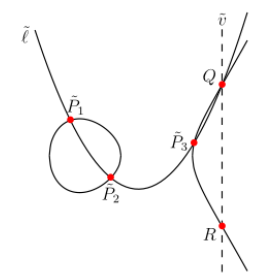
\includegraphics[width=0.32\linewidth]{98_Pictures/Chapter_03/divisorreduction}
	\caption[Illustration of Divisor reduction]{Illustration of divisor reduction using the Riemann-Roch Theorem based on \refExample{example:divisorreductionwithriemanroch} }
	\label{fig:divisorreduction}
\end{figure}


Using the one-to-one correspondence between the divisor
class group \mathFormulaPicardGroupWithIndexPar{E}{0} and the fact that points on $E$ has the group homomorphisms $P \mapsto (P) - (\mathFormulaEllipticCurvePointAtInfinity)$ we are now able to describe the chord-and-tangent rule without divisors or the definition of the divisor class group. 

Thus, within the elliptic curve setting, we can simply talk about
the group elements being points, rather than divisors. We note that however 
for other curves of higher genus or general abelian varieties this does not happen; group elements are no longer points, but rather divisor classes in \mathFormulaPicardGroupWithIndexPar{E}{0} with multiple elements in their support. 

Despite the abstraction presented above, the language of divisors is essential in the description of elliptic curve pairings, where the objective is to compute very large degree functions on $E$ with prescribed divisors, and then evaluate these functions at other divisors.  Such function evaluation can be described as in \refEquation{eq:ch1.evaulatingfatdivisors}. 

\insertEquationEnvironmentWithLabel{
	f(D) = \Pi_{P \in E}^{} f(P)^{n_P}/
}{eq:ch1.evaulatingfatdivisors}
where $f \in \FieldF_q(E)$ and divisor $D = \sum_{P \in E} n_P (E)$ has a natural definition, provided by divisors $(f)$ and $D$'s disjoint supports. The stipulation of disjoint supports is clearly necessary for $f(D)$ to be non-trivial since $P \in supp((f))$ imlies $P$ is a zero or pole of $f$ on $E$, meaning $f(P)^{n_P}$  is either zero or infinity respectively.



\begin{example}
%\todo{Example 3.2.4}
%\info{rephrase}
Consider $E/\mathbb{F}_{163} : y^2 = x^3 - x - 2$, with $P = (43, 154)$, $Q = (46, 38)$, $R = (12, 35)$ and $S = (5, 66)$ all on $E$. Let $\ell_{P,Q}$, $\ell_{P,P}$ and $\ell_{Q,Q}$ be the lines joining $P$ and $Q$, tangent to $P$, and tangent to $Q$ on $E$ respectively, computed as $\ell_{P,Q} : y + 93x + 85$, $\ell_{P,P} : y + 127x + 90$, $\ell_{Q,Q} : y + 13x + 16$. Let $D_1 = 2(R) + (S)$, $D_2 = 3(R) - 3(S)$ and $D_3 = (R) + (S) - 2(O)$. We can compute $\ell_{P,Q}(D_1) = (y_R + 93x_R + 85)^2(y_S + 93x_S + 85) = 122$, or $\ell_{P,P}(D_2) = (y_R + 127x_R + 90)^3/(y_S + 127x_S + 90)^3 = 53$, but we can not evaluate any of these functions at $D_3$, since $O \in \text{supp}(D_3)$, and $O$ is also in the supports of $(\ell_{P,Q})$, $(\ell_{P,P})$, $(\ell_{Q,Q})$. Let $\ell'_{P,P} = 17\ell_{P,P}$ so that $\ell'_{P,P} = 17y + 40x + 63$, and that $\ell'_{P,P}(D_2) = (17y_R + 40x_R + 63)^3/(17y_S + 40x_S + 63)^3 = 53 = \ell_{P,P}(D_2)$. This is true in general, i.e.\ that if $g = cf$ for some constant $c \in \mathbb{F}_q$, then $f(D) = g(D)$. If $D$ has degree zero; the constant $c$ will cancel out because $\deg(D) = 0$ implies the numerator and denominator of $f(D)$ (identically $g(D)$) have the same total degree.
\label{example:324}	
\end{example}

We conclude the current subsection with \refExample{example:324} by acknowledging in general  that if $g = cf$ for some constant $c \in \overline{\FieldF}_{q}$, then $f(D) = g(D)$. If $D$ has the constant $c$ will cancel out because $Deg(D) = 0$ implies the numerator and denominator of $f(D)$ have the same total degree.


In the following \refSection{sec:ch1.ellipticcurvesaspairinggroups} we are discussing cryptographic pairings as bilinear maps from two elliptic curve groups to a third (finite field) group,  \mathFormulaObject{e: \mathFormulaBilinearMapBetweenGroups{1}{2}{T}}, based on \cite{theory.pairings.for.beginners, menezes2004ECC,Menezes1993}.  As we will see, to be able to define a useful pairing on \mathFormulaObject{\GG_1} and \mathFormulaObject{\GG_2} we must be able to define more than one subgroup in the $r$-torsion of $E$ where the most useful case from the  cryptographic perspective will be when $r$ is a large prime. 
